
Due to the difference in wordsize between the old and new communication unit, a compatibility layer is added to allow other existing code to remain unchanged.

\figurename~\ref{fig:overview-lundal} shows the changes to the hardware platform.
The old COM40 unit has been replaced by a new communication unit and a compatibility layer.
The compatibility layer is needed because the old COM40 unit was based on 64-bit data while PCI Express uses 32-bit data.
\todo{blergh}

\begin{figure}[!ht]
    \centering
    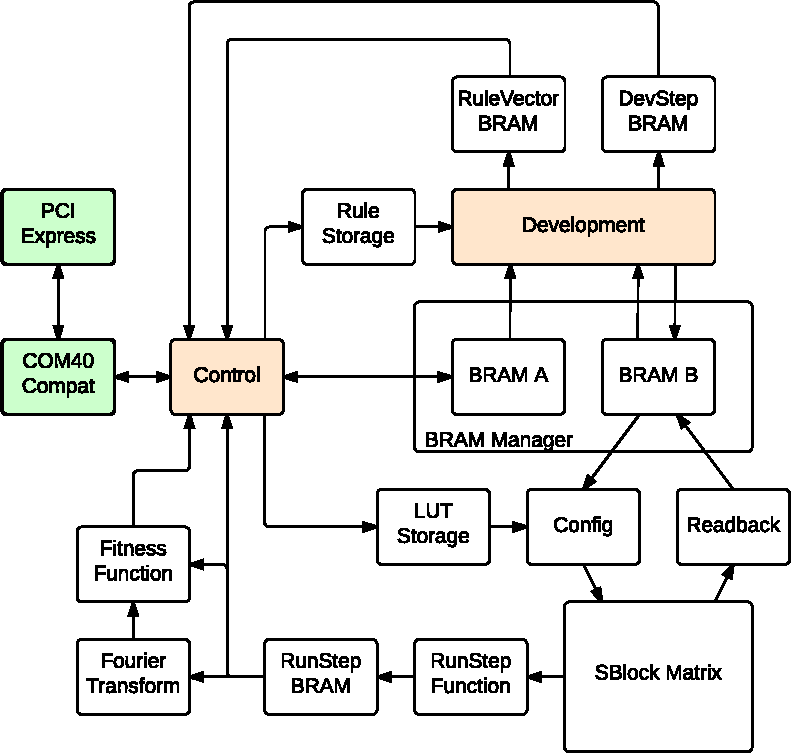
\includegraphics[width=0.48\textwidth]{figures/overview-lundal}
    \caption{High-level block diagram of the current hardware platform. Additions are highlighted in green.}
    \label{fig:overview-lundal}
\end{figure}

The communication unit has internal data buffers.

On the software side, the api uses linux' built-in drivers for PCI Express.

\subsection{Overview}

The new communication unit is based on Xilinx' reference PCI Express programmed io design.
It consists of the Xilinx PCI Express endpoint core, reception and transmission engines, data buffers, and a special request handler, as shown in \figurename~\ref{fig:details-communication}.

\begin{figure}[!ht]
    \centering
    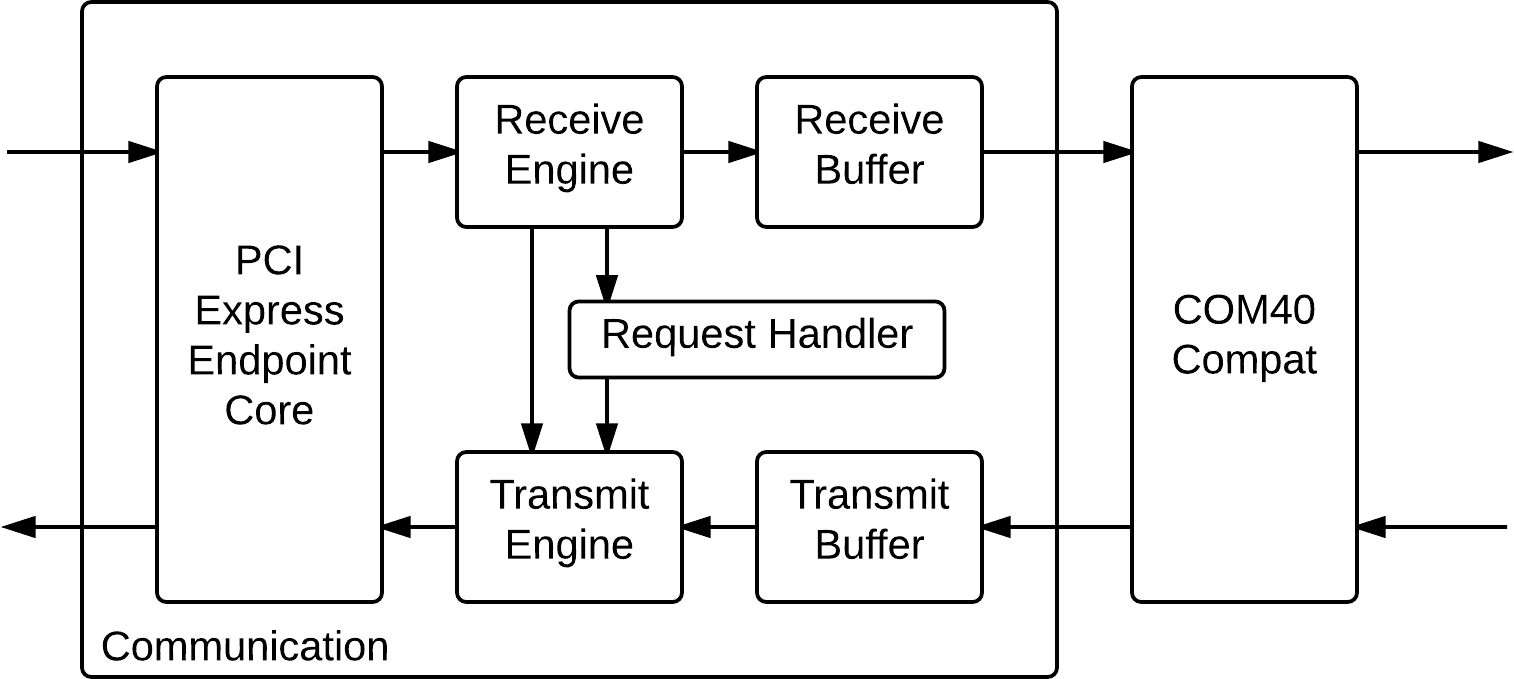
\includegraphics[width=0.48\textwidth]{figures/details-communication}
    \caption{Detailed block-diagram of the PCI Express communication module.}
    \label{fig:details-communication}
\end{figure}

The endpoint core handles all three PCI Express layers, and presents transaction layer packets (TLPs) on an AXI4-Stream interface \cite{ug672}.
The reception engine is responsible for parsing TLPs and either writing received data to the reception buffer or notifying the transmission engine about a read request.
The transmission engine is responsible for building TLPs to respond to read requests, using data from the transmission buffer.
The request handler listens to the read requests provided by the reception engine, and can override the transmission engine to answer special requests.
Those currently implemented are requests for amount of space or data in both buffers.

\subsection{Reception engine}

The reception engine is implemented as a simple state machine, as shown in \figurename~\ref{fig:statemachine-receive}.

\begin{figure}[!ht]
    \centering
    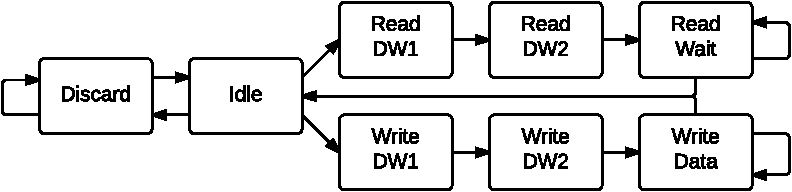
\includegraphics[width=0.48\textwidth]{figures/statemachine-receive}
    \caption{State machine for the reception engine.}
    \label{fig:statemachine-receive}
\end{figure}

Until the endpoint core presents valid data, the state machine remains in idle.
When it does, the data is stored, and the TLP type is checked.
If it is a read or write request, the state machine continues down the corresponding path, otherwise the remaining data is discarded.

\todo{describe reception engine}

\subsection{Transmission engine}

The transmission engine is implemented as a simple state machine, as shown in \figurename~\ref{fig:statemachine-transmit}.

\begin{figure}[!ht]
    \centering
    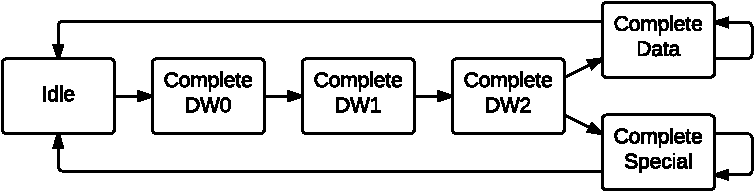
\includegraphics[width=0.48\textwidth]{figures/statemachine-transmit}
    \caption{State machine for the transmission engine.}
    \label{fig:statemachine-transmit}
\end{figure}

Until the reception engine signals a read request, the state machine remains in idle.

\todo{describe transmission engine}

\subsection{Buffers}

\todo{describe fifo buffers}

\begin{figure}[!ht]
    \centering
    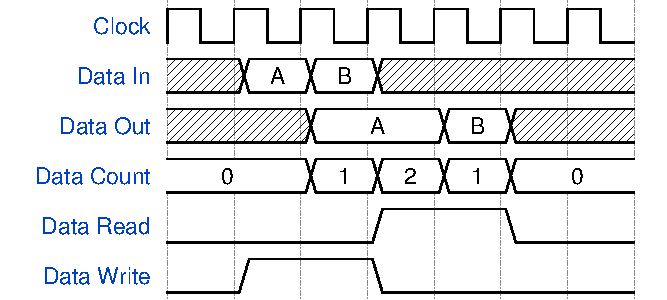
\includegraphics[width=0.40\textwidth]{figures/wavediagram-fifo}
    \caption{Wave diagram for the FIFO buffer, showing two consecutive writes followed by two consecutive reads.}
    \label{fig:wavediagram-fifo}
\end{figure}

Notice how the read signal needs to be asserted before the clock tick when data is read to ensure correct consecutive reads.
This is due to the BRAM used in the FIFO, which updates at clock ticks.
Therefore, the address has to be updated before the clock tick (by the read signal) to have correct data available for a read in the following cycle.

\todo{item chose native linux driver, files under /sys/devices/pci}
